\documentclass[12pt,a4paper]{article} 
\usepackage[portuguese]{babel}
\usepackage[utf8]{inputenc}
\usepackage{adjustbox}
\usepackage{amsmath} 
\usepackage{graphicx}
\usepackage{booktabs}
\usepackage{float}
\begin{document}
\setcounter{figure}{4}
\setcounter{section}{3}
\setcounter{page}{5}
\section{Relatório}
\subsection{Introdução}
A maior aplicação do diodo Zener reside na regulação de tensão de saída de fontes de alimentação. Através da utilização do diodo Zener, em conjunto com um resistor, pode-se conseguir que uma fonte de alimentação forneça tensão praticamente constante à carga. O comportamento do diodo Zener na região de ruptura permite a montagem de circuitos reguladores de tensão, que serão extremamente utéis para a fontes de corrente contínua, a fim de reduzir o fator de ripple destas, assim como ilustrado na Figura~\ref{fig:esquema_tensao}.

\begin{figure}[htpb]
  \centering
  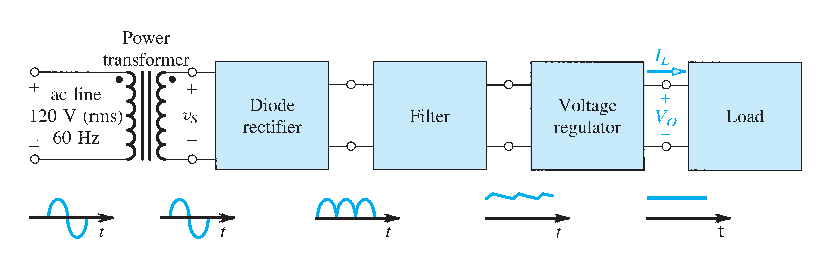
\includegraphics[width=0.8\linewidth]{./blocotransformador.pdf}
  \caption{Diagrama de blocos de uma fonte \emph{DC}.}
  \label{fig:esquema_tensao}
\end{figure}
A Figura~\ref{fig:breakdown} nos mostra detalhes da operação do diodo na região de ruptura. Observamos a existência de uma resistência dinâmica, $r_z$, o que implicará que a tensão que será aplicada na carga, $V_o$, terá uma pequena dependência na fonte de tensão, $V_s$. Em outras palavras, esperamos que se $V_s$ aumente, $V_o$ também será acrescido de um pequeno valor. O parâmetro que relaciona a variação de $V_o$ e de $V_s$ é chamado de regulação de linha.

Usando o raciocínio análogo ao parágrafo anterior, podemos relacionar a variação na  corrente da carga e na tensão de saída, dado que temos uma resistência dinâmica $r_z$. No entanto, também há a possibilidade de pensarmos em termos de resistência, já que $i_l= \frac{V_o}{R_l}$. Logo, teremos uma pequena dependência entre a resistência da carga, $R_l$, e a tensão da carga $V_o$. O parâmetro que relaciona a variação de $V-o$ e $i_l$ é chamado de regulação de carga. 

Neste experimento, estudaremos ambos os parâmetros e ainda exploraremos um componente mais sofisticado para regulagem de tensão, um circuito integrado da família $78xx$. O circuito integrado $7805$ é um regulador linear de tensão, e será utilizado em diversas configurações, cada qual com sua própria aplicação. Um regulador linear tensão, garante que se a tensão é garantidamente maior que um certo valor, um outro valor, mais baixo, será dado como saída.

\begin{figure}[htpb]
  \centering
  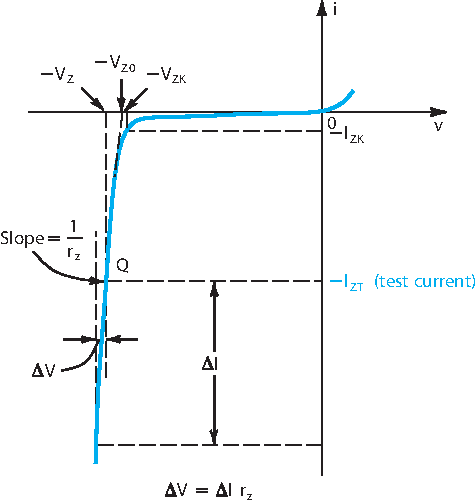
\includegraphics[width=0.6\linewidth]{breakdown_region.pdf}
  \caption{Relação detalhada da corrente e tensão de um Diodo Zener operando na região de ruptura.}
  \label{fig:breakdown}
\end{figure}

\newpage
\subsection{Análises}
%Exp1
Para $V_{in}$:

\begin{align*}
V_{medio} = 19.3 V \\
V_{rms} = 140 mV \\
V_{min} = 19.1 V \\
V_{max} = 19.7 V 
\end{align*}

Para $V_{out}$:
\begin{align*}
V_{medio} = 8.6 V \\
V_{rms} = 140 mV \\
V_{min} = 8.4 V \\
V_{max} = 8.8 V 
\end{align*}
\begin{figure}[htpb]
  \centering
  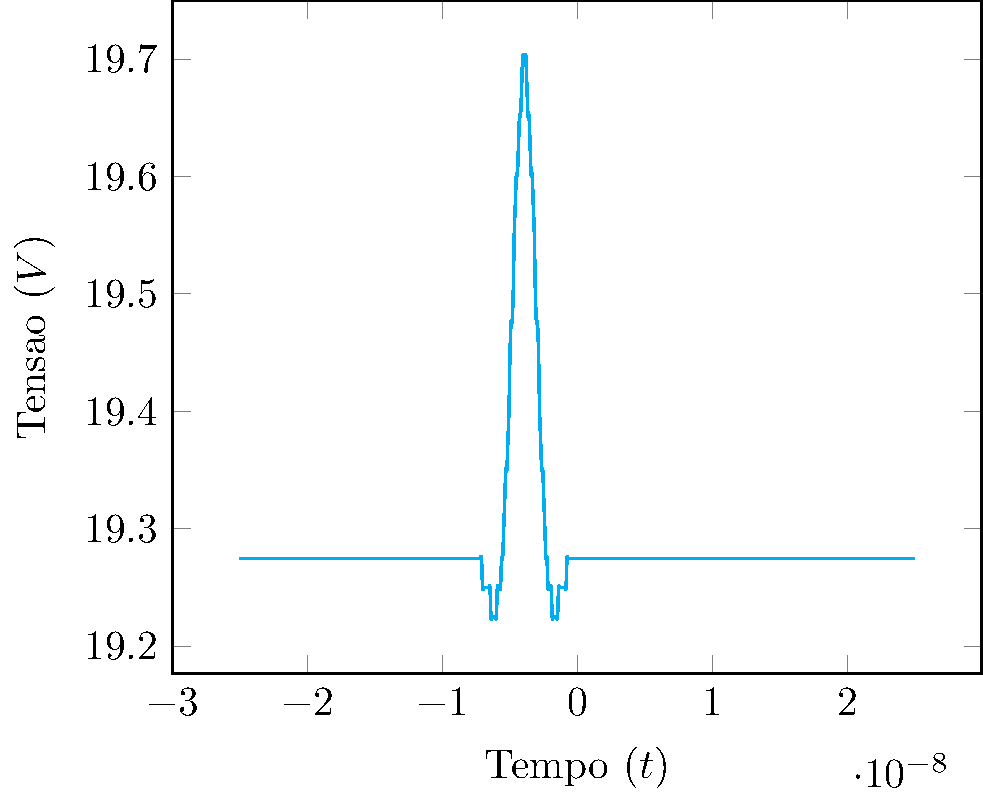
\includegraphics[width=0.8\linewidth]{./exp1/entrada_exp1.pdf}
\caption{}
  \label{fig:./exp1/entrada_exp1}
\end{figure}
\begin{figure}[htpb]
  \centering
  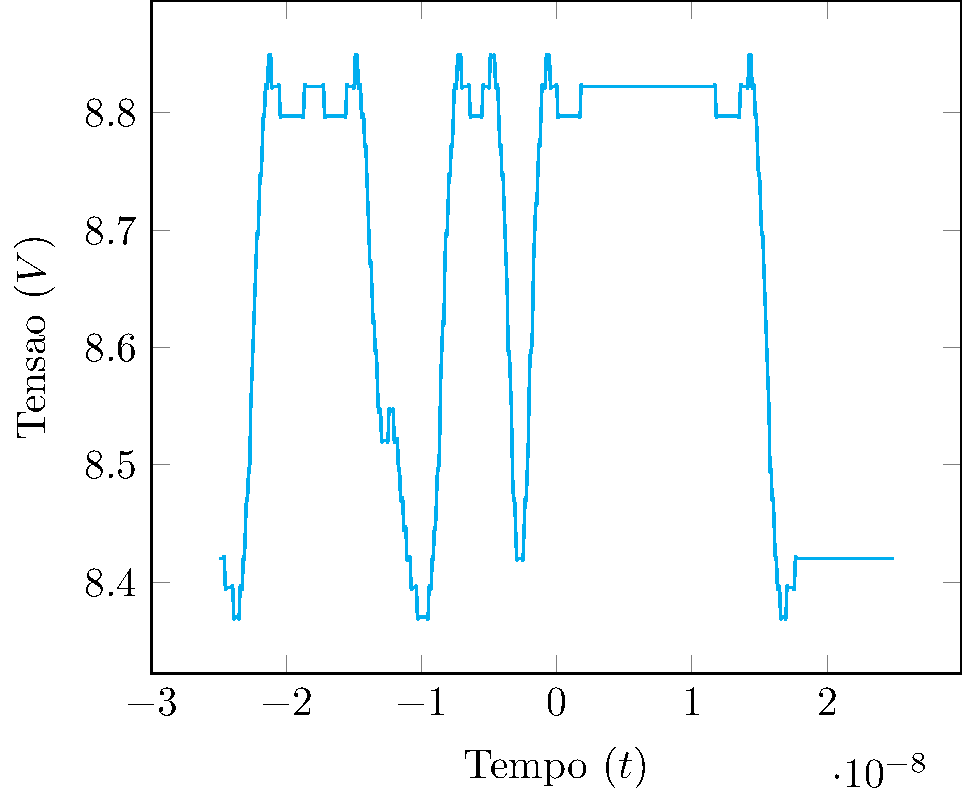
\includegraphics[width=0.8\linewidth]{./exp1/saida_exp1.pdf}
\caption{}
  \label{fig:./exp1/saida_exp1.pdf}
\end{figure}
%exp2
Para $V_{in}$:
\begin{align*}
V_{medio} = 19.5 V \\
V_{rms} = 90mV \\
V_{min} = 19.2 V \\
V_{max} = 19.7 V 
\end{align*}

Para $V_{out}$:
\begin{align*}
V_{medio} = 4.4 V \\
V_{rms} = 60 mV \\
V_{min} = 4.4 V \\
V_{max} = 4.8 V 
\end{align*}

\begin{figure}[htpb]
  \centering
  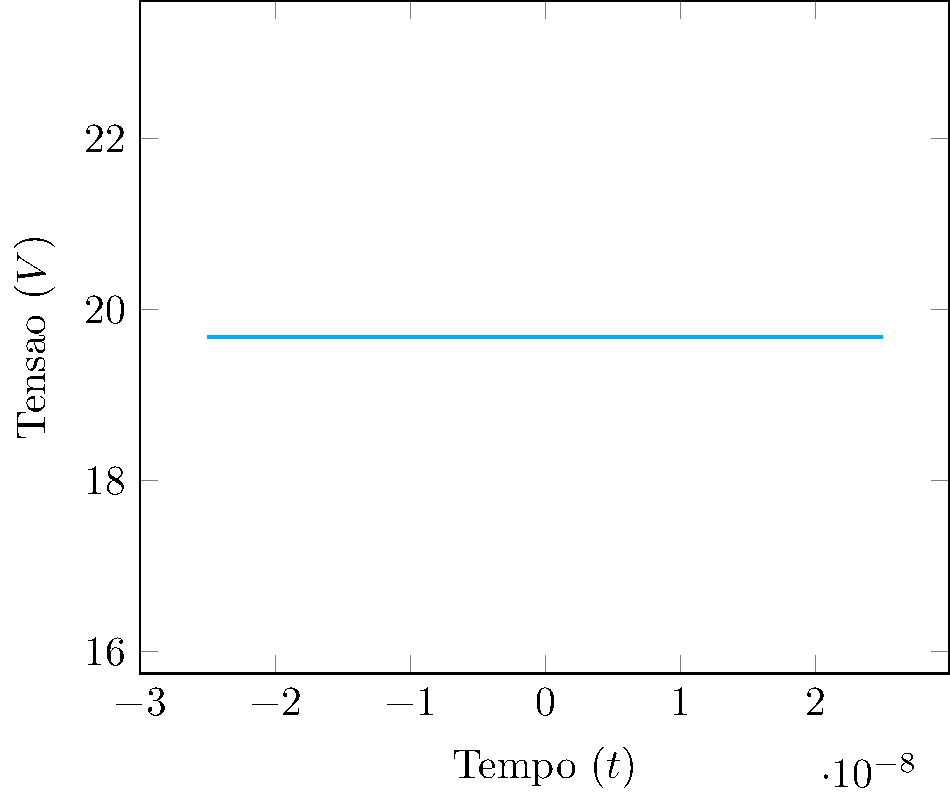
\includegraphics[width=0.8\linewidth]{./exp2/entrada_exp2.pdf}
  \caption{}
  \label{fig:./exp2/entrada_exp2}
\end{figure}
\begin{figure}[htpb]
  \centering
  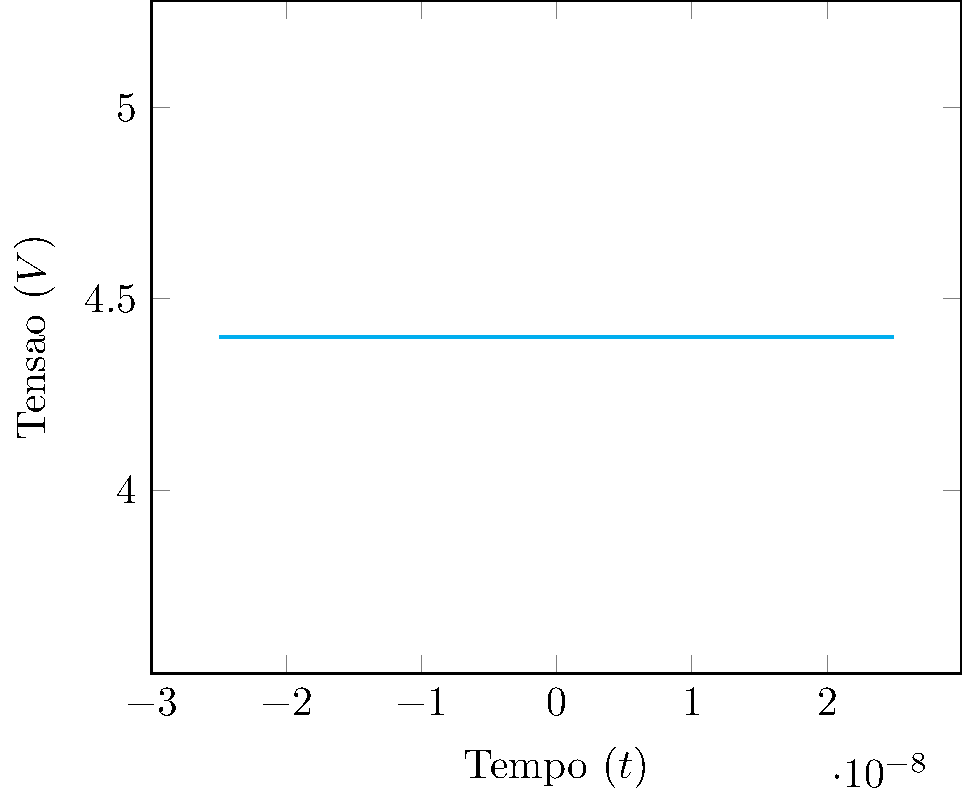
\includegraphics[width=0.8\linewidth]{./exp2/saida_exp2.pdf}
  \caption{}
  \label{fig:./exp2/saida_exp2}
\end{figure}
%exp3 
\begin{table}[htpb]
  \centering
  \caption{caption}
  \label{tab:label}
  \begin{tabular}{c c c c}
    \toprule
    $[\Omega]$ & Médio $[V]$ & Mínimo $[V]$  &  Máximo $[V]$\\ \midrule
   100  & $320 \times 10^{-3}$ & $200 \times 10^{-3}$& $400 \times 10^{-3}$ \\\midrule
   470& 2.3& 2.2& 2.4 \\\midrule
   820& 4.15& 4& 4.2 \\ \bottomrule 
  \end{tabular}
\end{table}
%exp4
\begin{table}[htpb]
  \centering
  \caption{caption}
  \label{tab:label}
  \begin{tabular}{c c c }
    \toprule
    $[\Omega]$ & $V_{l} [V]$&$i_l [mA]$  \\ \midrule
   47& 20.35& 111.5 \\\midrule
   100& 2.3& 56.1 \\\midrule
  \end{tabular}
\end{table}

\newpage
\subsection{Discussões}
\newpage
\subsection{Conclusão} \end{document}
